% !TEX root = knottedMain.tex
\documentclass[varwidth=\maxdimen]{standalone}

\usepackage{mathtools,amssymb,mathrsfs,dutchcal,upgreek,faktor,accents,etoolbox,multicol}
\usepackage[dvipsnames]{xcolor}
\definecolor{mygreen}{RGB}{	8,156,79 }
\usepackage{tikz,tikz-cd}
\usetikzlibrary{patterns,knots,arrows.meta,decorations.markings}
\tikzset{>={Straight Barb[scale=0.85]}}
\tikzcdset{
  cells={font=\everymath\expandafter{\the\everymath\displaystyle}},
  arrow style=tikz,
  diagrams={>={Straight Barb[scale=0.85]}},
  every label/.append style = {font = \small}
}


\begin{document}
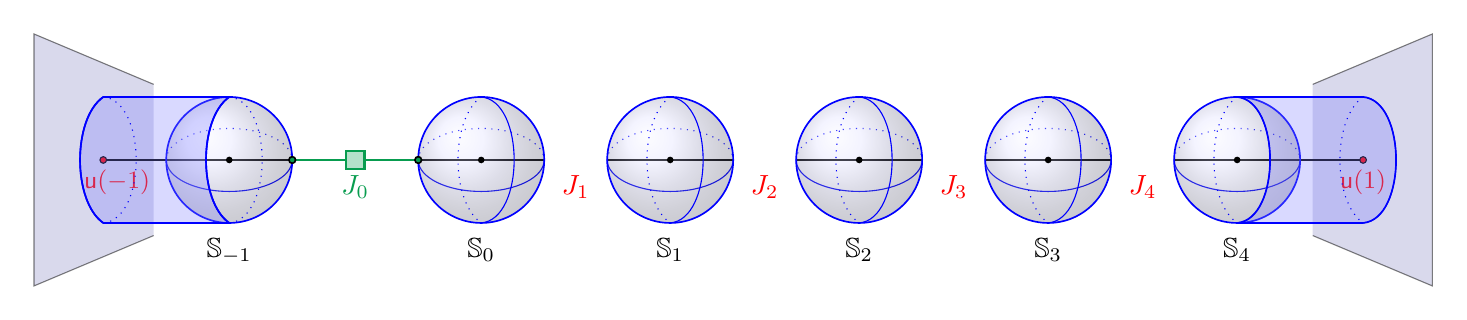
\begin{tikzpicture}[scale=0.8]
    \clip (-2.2,-2.1) rectangle (20.2,2.1);
    % boundary of M
    \fill[blue!50!black,opacity=0.15,draw=black,draw opacity=0.5]
        (18.2,-1.2) -- (20.1,-2) -- (20.1,2) --  (18.2,1.2) ;
    \fill[blue!50!black,opacity=0.15,draw=black,draw opacity=0.5]
        (-.2,1.2) -- (-2.1,2) -- (-2.1,-2) -- (-.2,-1.2) ;
    \draw[semithick]
        (-1,0) -- (2,0) 
        (4,0) -- (6,0) 
        (7,0) -- (9,0) 
        (10,0) -- (12,0) 
        (13,0) -- (15,0) 
        (16,0) -- (19,0) ;
    \draw[color=red, dashed,draw opacity=0]
        (6,0) -- (7,0) node[pos=0.5,below=2pt]{$J_1$}
        (9,0) -- (10,0) node[pos=0.5,below=2pt]{$J_2$}
        (12,0) -- (13,0) node[pos=0.5,below=2pt]{$J_3$}
        (15,0) -- (16,0) node[pos=0.5,below=2pt]{$J_4$};
    \fill[red,draw=black]
        (-1,0) circle (1.5pt) (-0.78,0) node[below]{\small$\mathsf{u}({-}1)$}
        (19,0) circle (1.5pt) node[below]{\small$\mathsf{u}(1)$};

    % spheres
    \foreach \y/\i/\j in {1/-1,5/0,8/1,11/2,14/3,17/4}{
        \draw[blue] (\y-1,0) arc (180:360:1cm and 0.5cm);
        \draw[blue,dotted] (\y-1,0) arc (180:0:1cm and 0.5cm);
        \shade[ball color=blue!20!,opacity=0.3] (\y,0) circle (1cm);
        \draw[blue,semithick] (\y,0) circle (1cm);
        \fill (\y,0) circle (1.5pt) %node[below]{\small$u_{\i}$}
        ;
        \draw (\y,-1) node[below=2pt]{$\mathbb{S}_{\i}$};
        }
    % cylinder left
    \fill[draw=blue,semithick,fill=blue!50!white,fill opacity=0.3]
        (-1,-1) -- (1,-1) to[out=145,in=-145, distance=0.6cm] 
        (1,1) -- (-1,1) to[out=-145,in=145, distance=0.6cm] (-1,-1);
    \draw[semithick,blue] 
        (-1,1) -- (1,1) 
        (1,-1) -- (-1,-1);
    % right cylinder
    \fill[draw=blue,semithick,fill=blue!50!white,fill opacity=0.3]
        (17,1) -- (19,1) to[out=-5,in=5, distance=0.7cm] 
        (19,-1) -- (17,-1) to[out=5,in=-5, distance=0.7cm] (17,1);
    % vertical arcs
    \foreach \x in {5,8,11,14,17,19}{
        \draw[blue]
            (\x,1) to[out=-5,in=5, distance=0.7cm] (\x,-1);
        \draw[blue,dotted]
            (\x,1) to[out=-145,in=145, distance=0.6cm] (\x,-1);
    }
    % vertical arcs on the first sphere
    \foreach \x in {-1,1}{
        \draw[blue,semithick]
            (\x,1) to[out=-145,in=145, distance=0.6cm] (\x,-1);
        \draw[blue, dotted]
            (\x,1) to[out=-5,in=5, distance=0.7cm] (\x,-1);
    }
    \draw[mygreen, thick]
            (2,0) -- (4,0) node[fill=mygreen!30,draw, pos=0.5]{}
            (3, 0) node[below=2pt]{$J_0$};
    \fill[mygreen,draw=black,semithick] 
        (2,0) circle (1.5pt) (4,0) circle (1.5pt);
\end{tikzpicture}

\end{document}